\chapter{Grundlagen}

\section{Software Design}

\subsection{Einführung}

Software-Design ist ein zentraler Aspekt der Softwareentwicklung, der maßgeblich den Erfolg und die Wartbarkeit eines Projekts beeinflusst. Verschiedene architektonische Patterns bieten Lösungen für wiederkehrende Probleme und helfen Entwicklern, robuste und skalierbare Anwendungen zu erstellen. Robert C. Martin, ein Pionier in der Software-Architektur, betont in seinem Buch \textit{Clean Architecture} die Bedeutung von guten Architekturen:

\begin{quote}
The goal of software architecture is to minimize the human resources required to build and maintain the required system. \autocite{martin:clean-architecture}
\end{quote}

Dieses Zitat unterstreicht, dass eine durchdachte Architektur nicht nur die Entwicklungszeit verkürzt, sondern auch die langfristige Wartung vereinfacht. In diesem Kontext werden im Folgenden zwei bedeutende architektonische Patterns vorgestellt, die im Rahmen der Projektdurchführung relevant sind: \ac{ddd} und Microservices.

\subsection{Architektonische Patterns und Ansätze}

\subsubsection{Microservices} \label{cha:grundlagen:swdesign:microservices}

Unter dem Begriff \textit{Microservices} versteht sich der Ansatz, ein Software-System als Orchestration mehrerer Dienste zu unterteilen. Jeder Dienst ist für eine Aufgabe des gesamten System-Kontexts verantwortlich und kann unabhängig von anderen Diensten als ein eigener Prozess laufen. \autocite{LewisFowler2024}

\subsubsection{Domain Driven Design} \label{cha:grundlagen:swdesign:ddd}

Das \textit{\ac{ddd}} ist eine Methodologie, die hauptsächlich bei komplexen Softwareprojekten zum Einsatz kommt. Es gehört weder zur Kategorie der Frameworks noch zu den architektonischen Patterns. Vielmehr ist es eng mit der Denkweise der Microservices, wie in Kapitel \ref{cha:grundlagen:swdesign:microservices} beschrieben, verbunden. Domain-driven Design konzentriert sich darauf, Aktivitäten und Prozesse aus dem realen Leben in die Softwareentwicklung zu abstrahieren. \autocite{LewisFowler2024}

\subsubsection{Onion-Architecture} \label{cha:grundlagen:swdesign:onion}

Die \textit{Onion-Architecture}, auch bekannt als \textit{Clean Architecture}, wurde von Jeffrey Palermo entwickelt und wird insbesondere für C\#-Projekte von Microsoft empfohlen. Sie zielt darauf ab, die typischen Probleme monolithischer Anwendungen, wie hohe Kopplung und geringe Wartbarkeit, zu vermeiden. Die Architektur visualisiert die Software als konzentrische Schichten, vergleichbar mit den Schichten einer Zwiebel. Folgende Abbildung stellt diesen Aufbau nochmals dar:

\begin{figure}[H]
    \centering
    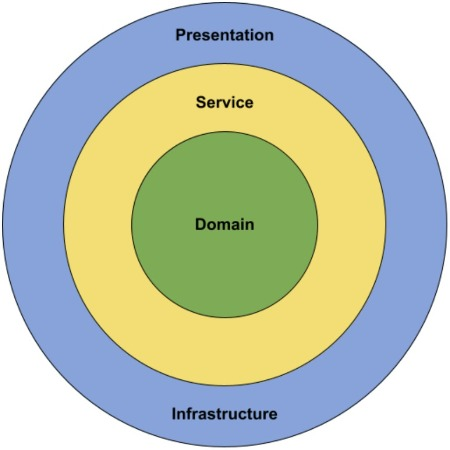
\includegraphics[width=.65\textwidth]{images/PrAR-Grundlagen-OnionArchitecture.jpeg}
    \caption{Bild Onion Architecture, nach \autocite{CodeMaze2024}}
    \label{fig:grundlagen:swdesign:onion}
\end{figure}

\newpage

Die Onion-Architecture gliedert sich in vier Hauptschichten:

\begin{itemize}
\item \textbf{Domain Layer:} Im Zentrum steht die Domäne, die Geschäftslogik und Geschäftsregeln beinhaltet und keinerlei Abhängigkeiten zu äußeren Schichten hat.
\item \textbf{Service Layer:} Diese Schicht enthält die Anwendungsspezifische Logik und nutzt die in der Domain Layer definierten Schnittstellen.
\item \textbf{Infrastructure Layer:} Hier befinden sich Implementierungen für Datenzugriff, Netzwerkkommunikation und andere externe Dienste.
\item \textbf{Presentation Layer:} Diese Schicht ist für die Benutzeroberfläche und die Präsentation der Daten verantwortlich.
\end{itemize}

Konzepte der Onion-Architecture fördern die Abhängigkeit von Abstraktionen (Interfaces) anstatt von konkreten Implementierungen. Diese Abhängigkeitsinversion erlaubt es, Implementierungen zur Laufzeit auszutauschen, was die Flexibilität und Erweiterbarkeit der Software erhöht.

Die Vorteile der Onion-Architecture sind:

\begin{itemize}
\item \textbf{Hohe Testbarkeit:} Da alle Schichten über definierte Schnittstellen kommunizieren, können einzelne Komponenten leicht isoliert und getestet werden.
\item \textbf{Klare Abhängigkeiten:} Abhängigkeiten fließen strikt in Richtung der zentralen Domänenschicht, wodurch höhere Schichten die Implementierungen der unteren Schichten verwenden können, aber nicht umgekehrt.
\item \textbf{Trennung von Geschäftslogik und Implementierungsdetails:} Die Geschäftslogik kann unabhängig von technischen Implementierungsdetails entwickelt werden. Notwendige Schnittstellen zu externen Systemen werden definiert, aber deren konkrete Implementierung wird in den äußeren Schichten gekapselt.
\end{itemize}

Diese Struktur ermöglicht es, komplexe Anwendungen modular zu entwickeln und erleichtert die Wartung und Weiterentwicklung der Software \autocite{CodeMaze2024}.

\subsection{Kollaboration mehrerer Dienste}

\subsubsection{Eventbasierte Architektur: Message Broker und Message Bus}

Eine eventbasierte Architektur ermöglicht es, Nachrichten schnell und flexibel zwischen mehreren Diensten auszutauschen. Ein verbreiteter Ansatz hierfür ist die Nutzung eines \textit{Message-Brokers}. Im Folgenden werden die vier grundlegenden Aspekte dieser Architektur beschrieben (vgl. \autocite{oreilly:mod-swarch}):
\begin{enumerate}
    \item \textbf{Initiierendes Event}: Ein \textit{Ereignis}, das den Event-Fluss anstößt und an einen Event-Kanal des Event-Brokers gesendet wird.
    \item \textbf{Event-Broker}: Ein \textit{Orchestrator}, der mehrere Kanäle verwaltet, auf denen Event-Prozessoren lauschen können.
    \item \textbf{Event-Prozessor}: Eine Einheit, die auf einem Kanal lauscht und ein eingehendes Event verarbeitet. Dabei kann ein neues (verarbeitetes) Event erzeugt und an einen anderen Kanal gesendet werden.
    \item \textbf{Das zu verarbeitende Event}: Ein Ereignis, das durch die beschriebenen Mechanismen verarbeitet oder erzeugt wird.
\end{enumerate}

\textbf{Vorteile}

\begin{enumerate}
    \item \textbf{Architektonische Erweiterbarkeit}: Events können vorläufig erzeugt und an den Message-Broker gesendet werden, ohne dass der Event-Prozessor bereits implementiert sein muss. Dies ermöglicht die spätere Implementierung des Prozessors.
    \item \textbf{Abkapselung}: Jedes Modul ist für seine eigene Funktionalität verantwortlich, während alles außerhalb Bestandteil anderer Module ist.
    \item \textbf{Skalierbarkeit}: Events können von mehreren (gleichen) Event-Prozessoren verarbeitet werden. Der Kanal fungiert als FIFO-Warteschlange und ermöglicht eine notwendige Synchronisation.
    \item \textbf{Asynchronität}: Die Kommunikation erfolgt asynchron, was die Entkopplung der Dienste und die Verbesserung der Systemleistung ermöglicht.
\end{enumerate}

\textbf{Nachteile}

\begin{enumerate}
    \item \textbf{(De-)Marshalling}: Nachrichten müssen in ein anderes Format (z.B. JSON, String, Byte-Array) konvertiert und wieder zurückkonvertiert werden. Dies kann die Performance beeinträchtigen.
    \item \textbf{Policies}: In einer traditionellen Message-Broking-Architektur kann theoretisch jeder auf einen Kanal \textit{subscriben}. Es gibt keine klaren Schichten zur Trennung der Zugriffsrechte.
    \item \textbf{Komplexität}: Das Management mehrerer Module und die Nachverfolgung von \textit{Event-Publishern} und \textit{Event-Subscriber} können schwierig sein.
\end{enumerate}

\subsubsection{RESTful APIs} \label{cha:grundlagen:collaboration:rest}

Für die Kommunikation und den Datenaustausch zwischen mehreren Diensten stehen verschiedene Kommunikations-Protokolle zur Verfügung. HTTP ist ein standardisiertes Kommunikationsprotokoll und ist in Bereichen der Web-Anwendungen weit verbreitet.

\ac{rest} definiert kein neues Kommunikationsprotokoll. Es ist ledigliche eine Sammlung von Architekturbeschränkungen und definiert Regeln, die der Entwickler befolgen muss, um eine Zustandslosigkeit in der Kommunikation zu erfüllen \autocite{RedHat2023}.

\section{Technologien}

Für die Implementierung wurden zahlreiche Technologien der Software-Entwicklung in Betracht gezogen. In diesem Abschnitt werden die für das Projekt relevanten Frameworks und Plattformen beschrieben.

\subsection{ASP.NET}

ASP.NET ist ein Open-Source-Web-Framework, das von Microsoft entwickelt wurde und die Erstellung moderner, skalierbarer und leistungsfähiger Webanwendungen ermöglicht. Zudem werden in ASP.NET moderne Webtechnologien und -standards unterstützt, wodurch sich die Entwicklung von interaktiven und responsiven Webanwendungen erleichtert. Dies schließt auch APIs und Echtzeit-Kommunikation ein, die für die Anwendung relevant sein könnten. Diese Merkmale ermöglichen es auch, die Anwendung modular zu ergänzen, indem externe APIs wie OpenStreetMaps oder andere Dienste einfach angebunden werden können.

\subsubsection{Entity Framework Core}

\ac{efcore} ist ein leichtgewichtiges, erweiterbares und Open-Source-\ac{orm} Framework für .NET, das entwickelt wurde, um den Datenzugriff und die Datenmanipulation in .NET-Anwendungen zu vereinfachen. \ac{efcore} bietet Datenbankunabhängigkeit, da es verschiedene Datenbanksysteme wie SQL Server, MySQL, PostgreSQL und SQLite unterstützt.

Ein weiterer Vorteil von \ac{efcore} ist Möglichkeit, das Datenbankschema aus konkreten Models über Source-Code zu generieren, ohne \textit{Create-Table} SQL-Statements schreiben zu müssen. \ac{efcore} bietet hierbei eine einfach zu verstehende \textit{Fluent-API} an. Zudem ermöglicht \ac{efcore} die einfache Verwaltung von Datenbankmigrationen, was es erlaubt, Änderungen am Datenmodell nachzuverfolgen und auf die Datenbank anzuwenden. Dies erleichtert die Wartung und Weiterentwicklung erheblich.

Ein zusätzliches Merkmal von \ac{efcore} ist die Integration von \ac{linq}, die es ermöglicht, komplexe Abfragen auf eine intuitive und typsichere Weise zu schreiben. Dies verbessert die Lesbarkeit und Wartbarkeit des Codes erheblich. Schließlich bietet \ac{efcore} verschiedene Mechanismen zur Performanceoptimierung, wie zum Beispiel asynchrone Abfragen und Caching-Strategien.

\subsection{Unity und Mobile-Apps}

Unity ist eine Plattform zur Entwicklung und Darstellung interaktiver 3D-Inhalte, die in vielen Bereichen wie Spieleentwicklung, Filmproduktion, Architekturvisualisierung und Virtual Reality (VR) eingesetzt wird. Sie ist eine der am weitesten verbreiteten Spiel-Engines weltweit und bietet eine Vielzahl an Werkzeugen und Funktionen, für das implementieren immersiver und realistischer Umgebungen.

Unity basiert auf einer Engine, die eine umfassende Sammlung von Software-Bibliotheken bereitstellt. Diese Bibliotheken ermöglichen die Verarbeitung von Grafiken, Physik, Sound und Benutzereingaben. Der Kern der Engine ist für die Rendern von 2D- und 3D-Grafiken verantwortlich, die in Echtzeit berechnet und auf dem Bildschirm angezeigt werden. Unity unterstützt die Programmiersprachen C\# und UnityScript (eine Art JavaScript, welche allerdings nicht mehr weiterentwickelt wird), wobei C\#  die primäre Sprache für die Entwicklung in Unity ist.

\subsubsection{AR-Foundation}

Für das Erstellen von Augmented-Reality Anwendungen bietet Unity unter der \textit{AR Foundation} grundlegende Bausteine an. Über vorgefertigte Projekt-Templates lässt sich eine funktionierende und ausführbare Demo-Anwendung für Android-Geräte generieren. Das AR Foundation Framework ermöglicht das Einbinden von Features wie beispielsweise Oberflächen-Erkennung, Objekt-, Bild- und Gesicht-Verfolgung sowie Sitzungs- und Geräte-Management \autocite{Unity2024}.

\subsubsection{Nützliche Bibliotheken}

\textit{Newtonsoft.Json.NET} ist eine in der Praxis verwendete Bibliothek in C\# bzw. .NET Anwendungen für das Serialisieren und Deserialisieren von Objekten im JSON-Format. Für die Verwendung in Unity-Anwendungen existiert ein GitHub-Fork (\textit{Json.Net.Unity3D}) und ermöglicht das Einbinden über eine \lstinline{.unitypackage} Datei. \autocite{SaladLab2024}

\textit{AR+GPS Location} ist eine Utility aus dem Unity-Asset-Store und ermöglicht eine Übersetzung von GPS-Koordinaten im Unity-Raum. Hierdurch können Objekte über die Angabe eines realen GPS-Standorts im Unity-Raum plaziert werden. Wenn die Anwendung an der realen Stelle des angegebenen GPS-Standorts geöffnet wird, wird das in Unity angelegte Objekt am richtigen Ort angezeigt. \autocite{ArGpsLocation}

\subsection{Svelte und Web-Apps}

\textbf{Svelte} ist ein modernes JavaScript-Framework zur Erstellung von Benutzeroberflächen. Im Gegensatz zu herkömmlichen Frameworks wie React oder Vue, die den Großteil ihrer Arbeit im Browser ausführen, verschiebt Svelte diese Arbeit in die Kompilierungsphase. Dies bedeutet, dass der Code während des Build-Prozesses in effizientes, optimiertes JavaScript umgewandelt wird, das direkt im Browser ausgeführt wird. Dadurch wird die Laufzeitbelastung erheblich reduziert, was zu einer besseren Performance und geringeren Ladezeiten führt \autocite{Svelte2024}.

Ein wesentlicher Vorteil von Svelte ist seine einfache Syntax, die es Entwicklern ermöglicht, reaktiven Code zu schreiben, ohne auf komplexe State-Management-Lösungen zurückzugreifen. Die Komponenten in Svelte bestehen aus HTML, CSS und JavaScript, was die Lernkurve für neue Benutzer verringert und die Entwicklungserfahrung vereinfacht \autocite{Svelte2024}.

\textbf{SvelteKit} ist ein Framework für den Aufbau von Svelte-Anwendungen. Es erweitert die Fähigkeiten von Svelte, indem es zusätzliche Werkzeuge und Funktionen bereitstellt, die speziell für die Entwicklung komplexer, leistungsstarker Webanwendungen notwendig sind. SvelteKit vereinfacht die Einrichtung und Strukturierung von Projekten und bietet Funktionen wie Routing, \ac{ssr}, statische Seitengenerierung und eine integrierte Entwicklungsumgebung \autocite{Svelte2024}.

\subsubsection{Vorteile}

Svelte integriert CSS-Styles direkt in die Komponenten mittels \textit{<style>-Tags}. Dies eliminiert die Notwendigkeit zusätzlicher Setups.

Alternativ kann auf bereits existierende CSS-Bibliotheken wie TailwindCSS zurückgegriffen werden. Standardmäßig werden Styles scoped angelegt, sodass keine Konflikte zwischen den Komponenten entstehen. Dies sorgt für eine sichere und wartbare Codebase einzelner Komponenten aufgrund der reduzierten Abhängigkeiten.

Svelte-Pages sind standardmäßig mit einem einfachen Prerendering ausgestattet, das sich über das Setzen eines Attributes steuern lässt. SvelteKit bietet zudem einfache Einstellungen, um verschiedene Startpfade für das Prerendering zu definieren, was die Flexibilität bei der Konfiguration erhöht.

Ein weiteres zentrales Feature von Svelte ist die Reaktivität. Durch das Definieren von sogenannten \textit{Reactive Statements} kann ein Ablauf beschrieben werden, der ausgeführt wird, wenn eine Abhängigkeit innerhalb dieses Blocks aktualisiert wird. Dies erleichtert das Management von Zustandsänderungen und sorgt für reaktive und dynamische Benutzeroberflächen.

Svelte besitzt eingebaute Prüfungen für Barrierefreiheit (\textit{Accessibility-Linting}), die auf offensichtliche und auch auf komplexere Probleme hinweisen. Dies unterstützt Entwickler dabei, von Anfang an barrierefreie Anwendungen zu erstellen.

Letztendlich reduziert sich die Menge des notwendigen Codes erheblich durch die deklarative Natur von Svelte. Diese führt zu einer klareren und übersichtlicheren Codebasis, was die Entwicklung und Wartung von Anwendungen vereinfacht \autocite{SvelteExperienceBespoyasov}.

\subsubsection{Nachteile}

Die Community-Größe von Svelte ist im Vergleich zu bekannteren JavaScript-Frameworks wie React oder Angular aufgrund der Neuheit des Frameworks noch relativ klein. Dies kann die Problemlösung erschweren, da einige Fehler möglicherweise nicht so gut dokumentiert oder gelöst sind und somit weniger Ressourcen auf Foren wie Stack Overflow zur Verfügung stehen.

Ein weiterer Nachteil ist das fehlende Entwickler-Tooling oder eine \ac{cli}. Bei Angular können Komponenten oder Dienste beispielsweise über die Angular \ac{cli} schnell und effizient erstellt werden. Diese Art von Tooling fehlt bei Svelte, was den Entwicklungsprozess etwas weniger komfortabel machen kann.

Zudem ist die Verfügbarkeit und Nutzbarkeit von bereits vorhandenen Libraries eingeschränkt. Obwohl diese Libraries nahtlos mit einem Paketmanager (z.B. npm von Node.js) installiert werden können, erfordert es oft zusätzlichen Aufwand, um sie in Svelte-Komponenten zu integrieren \autocite{SvelteVsSvelteKit2023}.